\documentclass[12pt,a4paper]{article}
\usepackage[style = authoryear, maxcitenames = 1, uniquelist=false, sorting = nyt, abbreviate = true, doi = true, backend = biber]{biblatex}
\usepackage[lmargin = 3.5cm, rmargin = 3.5cm, tmargin = 2.5cm, bmargin = 2.5cm]{geometry}
\usepackage[onehalfspacing]{setspace}
\usepackage{graphicx}
\usepackage{hyperref}
\usepackage{times}
\usepackage{csquotes}
\usepackage[UKenglish]{babel}
\usepackage[textsize=tiny]{todonotes}
\usepackage[acronym]{glossaries}
\usepackage{soul} % for command \hl
\usepackage{pdfpages} % to insert pdf docs
\usepackage{csvsimple} % to import .csv files as tables
\usepackage{siunitx}
\usepackage{tikz}
\usepackage{caption} 
\usepackage{float}
\usepackage[T1]{fontenc}
\usepackage[parfill]{parskip}
\captionsetup[table]{skip=10pt} % more space between table and caption

\AtBeginBibliography{\small}
\addbibresource{main_sources.bib}
\setlength{\parindent}{0cm}
\setlength{\parskip}{0.172cm}
\setlength{\marginparwidth}{3.5cm} % make todonotes wider
\newcommand{\todoleft}[1]{{\reversemarginpar \todo{#1}}}


%%%%%%%%%%%%%%%%%%%%%%%%%%%%%%%%%%%%%%%%%%%%%%%%%%%%%%%%%%%%%%%%%%
\begin{document}
\def\findate{24.07.2024}


%title page
\thispagestyle{empty}
\begin{center}
    \Large{University of Innsbruck \\ Faculty of Mathematics, Computer Science and Physics} \\
    \vspace{3mm}
    \large{Institute for Theoretical Physics}
    \vspace{10mm}

    \includegraphics[width = 0.6 \linewidth]{logo.jpg}

    \vspace{10mm}
    \Large{Bachelor Thesis} \\
    \large{submitted for the degree of} \\
    \Large{Bachelor of Science} \\
    \vspace{10mm}
    \LARGE{\textbf{An information-theoretical approach to internal models in a Partially Observable Markov Decision Process}} \\
    \vspace{10mm}

    \large{by \\ Lukas Prader \\ Matriculation Nr.: 12115058 \\ SE Seminar with Bachelor Thesis}
\end{center}

\vspace{30mm}
\begin{tabular}{ll}
    \large{Submission Date:} & \large{\findate}                          \\
    \large{Supervisors:}     & \large{Alexander Vining, Hans J  Briegel} \\
\end{tabular}


\newpage
\thispagestyle{empty}
\begin{abstract}
    \noindent Intelligent biological agents are able to make sense of their environment and learn to act in it.
    In order to accurately replicate these behaviours and other complex phenomena in artificial agents, we need better models of the information processing happening in biological organisms.
    When only provided with partial information about a system, current artificial agents rely on sufficiently complex internal structures (i.e. a sufficient number of optimizable parameters) to enable them to learn complex tasks, yet the question remains how these internal structures come to be.
    In this work, an information theoretical approach to internal model generation was explored with a simple delayed action task.
    The results show great potential for the framework to enable dynamic internal model generation, with further analysis necessary concerning the scenario of an agent estimating information theoretical quantities from finite samples.\\

    \noindent Keywords: reinforcement learning, information theory, Partially Observable Markov Decision Process, internal model
\end{abstract}

\pagenumbering{roman}

\newpage
\tableofcontents
\thispagestyle{empty}
\newpage
\pagenumbering{arabic}

\section{Introduction} \label{sec:introduction}
The rise of artificial intelligence in recent years has produced new research trying to create complex models able to perform intelligent tasks.
In many disciplines it has been shown that there are so-called emergent phenomena, which are not easily explained by lower-level fundamental laws, requiring additional concepts to accurately explain them \autocite{anderson1972more}.
Exactly how these complex phenomena can emerge from the set of currently known fundamental laws is an ongoing field of research, with interdisciplinary approaches taking from the fields of physics, chemistry, biology, psychology, philosophy computer science and others.

Research into  so-called complex adaptive systems, for example connected to biology, aims to understand the emergence of intelligent and adaptive behaviour in biological organisms.
Gaining insight into the mechanisms which enable biological systems to exhibit complex behaviour can in turn be used to improve the ways in which we attempt to create systems capable of these behaviours ourselves.

Complex system research can thus provide valuable insights into the emergence of intelligent behaviour, which also includes processes connected to adaptive behaviour and learning in animals.
Works by the likes of Pavlov and Skinner have probed into the mechanisms that influence behavioural patterns in animals \autocite{pavlov1906scientific, skinner1957experimental}.
Exactly how conditionable behaviour like this can emerge just from interaction with the environment is still not fully understood.

Information theory has been fundamental in furthering our understanding of such complex processes.
With the work of Shannon \autocite{shannon1948} as a basis, modern information theory has enabled researchers to quantify correlations and changes in complexity of dynamic systems.
It has successfully been applied to many examples in behavioural biology, such as looking into the collective behaviour of ants, information exchange in slime moulds and group behaviour in bat populations \autocite{kim2021informational}.

Information theory can also be used to examine how biological agents, such as animals, acquire an understanding of their surroundings in order to then act in response, a so-called internal model of their environment.
Current approaches to create artificial agents able to learn certain behaviours rely on trial and error to find the number of parameters necessary to explain the complexity of a given environment, especially if only limited information about an environment is available to the agent.

Real life organisms do not seem to be limited as much, still being able to infer information about their environment even with limited information at their disposal.
Logical conclusions based on indirectly connected information, called transitive inference, has been shown in multiple animals such as pigeons, honey bees, rats and others \autocite{vasconcelos2008transitive}.
Here, animals are able to infer the relations between stimuli only with information about other stimuli and their relations to each other.
Also in the field of Artificial General Intelligence, tests like the ARC test set \autocite{chollet2019measure} show that current state-of-the-art machine learning models are not able to replicate reasoning tasks routinely performed by humans \autocite{johnson2021fast}.

Crutchfield and Feldman have proposed information theoretical quantities able to explain processes of inference for complex systems \autocite{crutchfield2003regularities}.
They can quantify the amount of "synchronization" a system has achieved in comparison to a different system (like an environment), which it can interact with.
This framework can provide tools which may enable an agent to autonomously modify the current internal model in order to more accurately reflect the processes of the observed environment.

This thesis aims to apply some of the quantities proposed by Crutchfield and Feldman to a simple example of an agent acting with partial information of its environment.
The goal is to show the capabilities of this framework to enable evaluation of the current internal model and subsequent improvements to accurately reflect the environment, even with only partial information available to the agent.
We will specifically examine how to determine if an internal model has reached sufficient complexity to explain the processes it observes and how this can be used to create an adequate internal model.

\newpage
\section{Methods} \label{sec:methods}

We will look at a small system related to behavioural biology, which can be modelled as a Markov Decision Process.
A Markov Decision Process (MDP) \autocite{bellman1957MDP} is defined by a set of states $S$, which are connected by transition probabilities, and a set of actions that an agent can perform in a given state.
These actions are determined by the agent's policy, commonly denoted with $\pi$.
One usually imposes the Markovian property, which implies that the transition probability from one state to the next only depends on the state itself and not the previous states of the system \autocite{cover1999elements}.

\subsection{The delayed action task} \label{ssec:delayed_action_mdp}
The system we will analyse is a delayed action task, which we want our agent to learn.
One can imagine a rat in a box, very similar to the aforementioned experiments by Skinner.
In this box, the rat observes a light switching on and off and has access to a button it can press.
The rat can obtain rewards, such as food, based on its actions. The light's state (on or off) changes in discrete time steps depending on the rat's actions.
In our setup, the rat receives a reward only if it presses the button at the correct time after the light turns on, specifically in the second time step.
This process can be visualized as the graph of a MDP, using three states and the possible transition probabilities as edges between them (Fig. \ref{fig:delayed_mdp}).

\begin{figure}[H]
    \centering
    % delayed action mdp
    \resizebox{0.5\linewidth}{!}{
        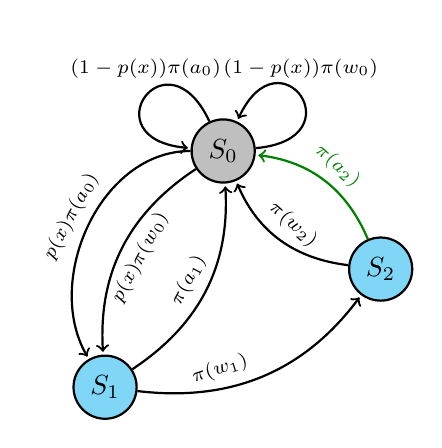
\begin{tikzpicture}[->,shorten >=1pt,auto,node distance=3cm,
                thick,main node/.style={circle,draw,font=\sffamily\Large\bfseries}]

            \node[fill=gray!50, circle, draw=black] (0) at (0,0) {$S_0$};
            \node[fill=cyan!50, circle, draw=black] (1) at (-1.5,-3) {$S_1$};
            \node[fill=cyan!50, circle, draw=black] (2) at (2,-1.5) {$S_2$};

            \path[every node/.style={font=\sffamily\scriptsize}]
            (0) edge [in=175,out=115, loop] node[above=3pt] {$(1-p(x)) \pi(a_0)$} (0)
            (0) edge [in=65,out=5, loop] node[above=3pt] {$(1-p(x)) \pi(w_0)$} (0)
            (0) edge [in=120,out=180] node[above, rotate=62] {$p(x) \pi(a_0)$} (1)
            (0) edge [bend right] node[below, rotate=62] {$p(x) \pi(w_0)$} (1)
            (1) edge [bend right] node[above, rotate=62] {$\pi(a_1)$} (0)
            (1) edge [bend right] node[rotate=18] {$\pi(w_1)$} (2)
            (2) edge [bend left] node[above, rotate=-42] {$\pi(w_2)$} (0)
            (2) edge [bend right, black!50!green] node[above, rotate=-42] {$\pi(a_2)$} (0);

        \end{tikzpicture}
    }
    \caption{\label{fig:delayed_mdp} Visualization of the delayed action MDP. Colours of the states describe the state of the light (grey = dark, blue = light) Probabilities coming from the agent policy, acting $a_i$ or waiting $w_i$ for a state with index $i$, are denoted with $\pi$. The probability of the light turning on in the dark state is given as $p(x)$.}
\end{figure}

In the most general case, the policy of the agent can be different in every state $S_i$.
We will define the policy to be a probability, with probabilities of choosing to either wait $\pi(w_i)$ or act and press the button $\pi(a_i)$. One can specify the policy only by defining the probability to act, consequently choosing the probability to wait as the inverse probability $1-\pi(a_i)$.
We will assume that the state of the light is fully determined by the agent's actions when being on, but if it is off, there is a probability of $p(x)$ for the light to turn on, independent of the agents action taken in the dark state.

The given MDP has two main properties, stationarity and irreducibility.
Being irreducible means that every state is reachable from every other state with positive probability in a finite number of steps \autocite{cover1999elements}, while stationarity implies that the transition probabilities do not change over time.
This is the case for our MDP, if we assume the policy to be fixed.

If we are specifically interested in the transitions for the states of the light, we can write the state transitions of this MDP into a state transition matrix $P$ (assuming some fixed policy $\pi$):
\begin{equation}
    \label{eq:P_mdp}
    P_{MDP} =
    \begin{bmatrix} 1 - p(x) & p(x) & 0            \\
                \pi(a_1) & 0    & 1 - \pi(a_1) \\
                1        & 0    & 0
    \end{bmatrix},
\end{equation}
with each row summing up to one.

One can see that the system reflected by this transition matrix does not capture the whole information about our initial system any more, ignoring the reward and the actions that do not directly influence the transitions of the light.

With the state transition matrix we can calculate the probability of ending up in a state in the next time step, given the probability of being in any of the states in the step before.
If we let the system transition for many time steps, the state distribution will converge to the so-called stationary distribution \autocite{cover1999elements}.
This stationary distribution $\mu$, a row vector by convention, satisfies the following equation:
\begin{equation}
    \label{eq:stationary_dist}
    \mu = P \mu.
\end{equation}

This means that $\mu$ can be calculated by finding the matrix eigenvector with eigenvalue 1.
The eigenvector should be re-scaled if necessary, such that the stationary distribution also has a sum of 1.

\subsection{Entropy and entropy rate} \label{ssec:entropy_rate}
Since we are interested in modelling an agent learning the task, we will treat it as a process generating observations.
In this way, we are able to analyse how an internal model can be formed, especially if there is no direct interaction to the task.
One can picture an observer just receiving the observations, without having any additional context to aid in interpretation.
The agent can observe parameters of the system, in particular the current state of the light and the action that was just performed.
Over multiple time steps, these observations will form sequences made up of symbols, which correspond to the particular state that was observed.
The sequences will have a symbol distribution dependent on the nature of the generating process, motivating the use of information theory to analyse the properties of these sequences.

The standard Shannon entropy,
\begin{equation}
    \label{eq:shannon_entropy}
    H = -\sum_{x \epsilon \mathcal{X}} p(x) \log p(x),
\end{equation}
is defined with the sum over all symbols $x$ in a given alphabet $\mathcal{X}$, $\log$ meaning the base two logarithm here, as well as in the rest of this thesis, implying "bits" as the unit of information.
Given a sequence, we can also calculate the entropy of tuples, which we will call blocks, of symbols.
We can define the block entropy $H(s^L)$ as the entropy of blocks of symbols with length $L$:
\begin{equation}
    \label{eq:block_entropy}
    H(s^L) = -\sum_{s_i^L \epsilon S^L} p(s_i^L) \log p(s_i^L),
\end{equation}
looking at all possible blocks $s_i^L$ of length $L$, given a set of symbols $S$.
One simple intuition to understand this is to think about the entropy of words.
Instead of calculating the entropy of the individual letters, we calculate the entropy of length $L$ words in a given sentence.

For a given block length, one can define the change of entropy at this length using the discrete derivative:
\begin{equation}
    \label{eq:entropy_change}
    \Delta H(s^L) = H(s^L) - H(s^{L-1}).
\end{equation}

This change in block entropy is equivalent to an estimate of the entropy rate $\hat{h}_\mu(L)$ at length $L$, which measures how random the system appears if only blocks up to length $L$ are observed.
For an infinitely long sequence, the change in entropy converges to the final entropy rate \autocite{crutchfield2003regularities}:
\begin{equation}
    \label{eq:entropy_rate_limit}
    h_\mu = \lim_{L \to \infty} \frac{H(s^L)}{L}.
\end{equation}

This entropy rate can be interpreted as the inherent randomness of sequences obtained from the generating process, stemming from the full complexity of the system.
It can also be shown that $\Delta H(s^L)$ decreases monotonically for increasing $L$, implying that a finite estimate of $h_\mu$ will tend to overestimate the randomness of an incoming sequence, and thus of the generating process \autocite{crutchfield2003regularities}.

For a stationary Markov Process, the final entropy rate can be calculated if the stationary distribution and the transition matrix are known \autocite{cover1999elements}:
\begin{equation}
    \label{eq:entropy_rate_MP}
    h_\mu = -\sum_i \mu_i \sum_j P_{ij} \log P_{ij}.
\end{equation}

\subsection{Synchronization and predictability gain} \label{ssec:synch_predgain}
Knowing how exactly $\Delta H(s^L)$ of a system converges to the final entropy rate $h_\mu$ provides information about the complexity and structure of the system.
Depending on the length of blocks used, the estimated complexity will be different from the true complexity of the system.
This opens the question of when an agent observing a sequence from a generating process can be said to have obtained all the information about the system.
At this point the agent would have all the information necessary to understand the nature of the generating process.
So-called "synchronization" is achieved once the discrete change in entropy is equal to the true final entropy rate of the system \autocite{crutchfield2003regularities}:
\begin{equation}
    \label{eq:synchronisation_equality}
    h_\mu - \Delta H(s^L) = 0.
\end{equation}
It means that there is no new information in blocks larger than $L$, for which synchronization was achieved.

This criterion depends on knowing the true entropy rate of the generating process, or at least having a very good estimate of it.
In general, this might not be feasible to obtain for an agent, especially since the agent will have no prior knowledge about the generating process, which it could use to estimate the entropy rate.

A different, although weaker condition to characterize synchronization is that the entropy rate has to be constant from then on.
This means that the second derivative $\Delta^2 H(s^L)$ will be 0.
We define
\begin{equation}
    \label{eq:predictability_gain}
    \Delta^2 H(s^L) = \Delta H(s^L) - \Delta H(s^{L-1}),
\end{equation}
also called predictability gain, which quantifies how much randomness is lost when using information of length $L$ blocks \autocite{crutchfield2003regularities}.
In order to sensibly define the predictability gain for $L=1$, one defines $\Delta H(s^0) = \log |S|$, using the number of symbols in $S$ defined by the cardinality $|S|$.
This is motivated by the idea that the randomness of the system is assumed to be maximal if no sequences have yet been observed \autocite{crutchfield2003regularities}.
It is important to note that for synchronization to be achieved, the predictability gain has to be zero for all following block lengths.
In some cases like periodic processes, it can happen that $\Delta^2 H(s^L)$ will be zero for some blocks, but different from zero for following blocks due to the periodic nature of the process \autocite{crutchfield2003regularities}.

\subsection{Observing the delayed action task} \label{ssec:observing_mdp}
In the case of the delayed action task (section \ref{ssec:delayed_action_mdp}), the ability for an agent to learn this task heavily depends on the type of information it has about the system.
If the agent is able to observe the true labels of each state, namely $S_0, S_1$ and $S_2$ (Fig. \ref{fig:obs_L_mdp}), it can easily find the optimal policy maximizing the reward.

\begin{figure}[H]
    \centering
    % delayed action mdp
    \resizebox{0.7\linewidth}{!}{
        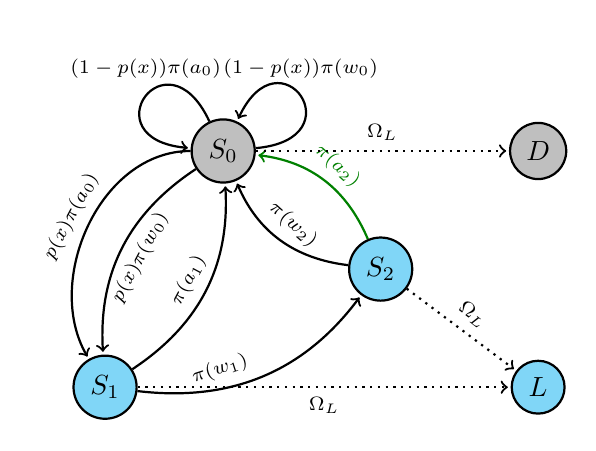
\begin{tikzpicture}[->,shorten >=1pt,auto,node distance=3cm,
                thick,main node/.style={circle,draw,font=\sffamily\Large\bfseries}]

            \node[fill=gray!50, circle, draw=black] (0) at (0,0) {$S_0$};
            \node[fill=cyan!50, circle, draw=black] (1) at (-1.5,-3) {$S_1$};
            \node[fill=cyan!50, circle, draw=black] (2) at (2,-1.5) {$S_2$};
            \node[fill=gray!50, circle, draw=black] (D) at (4,0) {$D$};
            \node[fill=cyan!50, circle, draw=black] (L) at (4,-3) {$L$};

            \path[every node/.style={font=\sffamily\scriptsize}]
            (0) edge [in=175,out=115, loop] node[above=3pt] {$(1-p(x)) \pi(a_0)$} (0)
            (0) edge [in=65,out=5, loop] node[above=3pt] {$(1-p(x)) \pi(w_0)$} (0)
            (0) edge [in=120,out=180] node[above, rotate=62] {$p(x) \pi(a_0)$} (1)
            (0) edge [bend right] node[below, rotate=62] {$p(x) \pi(w_0)$} (1)
            (1) edge [bend right] node[above, rotate=62] {$\pi(a_1)$} (0)
            (1) edge [bend right] node[rotate=18] {$\pi(w_1)$} (2)
            (2) edge [bend left] node[above, rotate=-42] {$\pi(w_2)$} (0)
            (2) edge [bend right, black!50!green] node[above, rotate=-42] {$\pi(a_2)$} (0)
            (0) edge [dotted] node[above] {$\Omega_L$} (D)
            (1) edge [dotted] node[below] {$\Omega_L$} (L)
            (2) edge [dotted] node[above, rotate=-38] {$\Omega_L$} (L);

        \end{tikzpicture}
    }
    \caption{\label{fig:obs_L_mdp} The process of reducing the delayed action task (Fig. \ref{fig:delayed_mdp}) to the observable light states using the mapping $\Omega_L$. One can see that $S_1$ and $S_2$ produce the same observation.}
\end{figure}

If the agent can only distinguish between light and dark states based on observations of the light, it can not distinguish $S_1$ and $S_2$, making it a Partially Observable Markov Decision Process (POMDP).
In this case, the agent will not be able to reach the optimal policy, since it can not distinguish the rewarded light state $S_2$ from the unrewarded $S_1$.
Yet, due to the temporal structure of the MDP, one can make a difference between $S_1$ and $S_2$ as soon as the prior state of the light is also known.
If the agent were able to use this information, it would again be in a position to distinguish $S_1$ and $S_2$, making it possible to learn the delayed action task once more.

This motivates the idea to use the measures shown in the previous sections, since they should be able to find this temporal correlation.
In particular, we should be able to show this temporal structure in the change of block entropy, so a different $\Delta H(s^L)$ for $L \leq 2$ and $L>2$.
We will thus analyse sequences of the original MDP, reduced to partial observations, and try to quantify the information encoded in them with higher block lengths.

In order to obtain these sequences, we have to first generate a sequence from the true MDP and then reduce the symbols to the partial observation we want to look at (i.e. Fig. \ref{fig:obs_L_mdp} for observing the light).
This reduction is performed by an observation mapping $\Omega_K$, with $K$ being the chosen observation.
Two main sources of information in this process are the state of the light ($L,D \to$ light, dark) and the actions taken by the agent ($A,W \to$ act, wait), which is why we will analyse the behaviour of both of them in the following sections.

\subsection{Quantity estimation}
Since information entropy and the quantities derived thereof use probabilities, their true values are results of using infinite samples.
Since this is not achievable for a real agent, we will have to use the estimated probabilities.
The agent can estimate the likelihood of a block by calculating the frequency of it in a given observation sequence, i.e. for the probability of a specific block $s_i^L$ we get
\begin{equation}
    \label{eq:prob_estimator}
    \hat{p}(s_i^L) = \frac{n(s_i^L)}{N},
\end{equation}
with $N$ being the total number of blocks of length $L$ in the given sequence.

As an illustrative example, we take the sequence D L L D L D.
For blocks of length 2, we get $DL$, $LL$, $LD$, $DL$ and $LD$.
From this, one could now calculate the frequencies of all possible blocks of length 2.
With the defined probability estimator, we can define the so-called plug-in-estimator for the block entropy:
\begin{equation}
    \label{eq:plug_in_block_ent}
    \hat{H}(s^L) = -\sum_{s_i^L \epsilon S^L} \hat{p}(s_i^L) \log \hat{p}(s_i^L),
\end{equation}
which we will use later to compare estimated values to the analytical results.

\newpage
\section{Results} \label{sec:results}

\subsection{Stationary distribution and partial models} \label{ssec:res_stationary_dist}
To be able to calculate the block entropy curve for the delayed action task, one first calculates the stationary distribution of the system.
Using equation (\ref{eq:stationary_dist}) with the transition matrix $P$ (\ref{eq:P_mdp}), we get the probabilities of encountering each state when observing the system at some random point in time:
\begin{equation}
    \label{eq:result_stationary_dist_mdp}
    \begin{split}
        \mu_{MDP} &= [p(S_0),\ p(S_1),\ p(S_2)] =       \\
        &=[\frac{1}{1 + p(x)(2-\pi(a_1))},\
        \frac{p(x)}{1 + p(x)(2-\pi(a_1))},\
        \frac{p(x)(1-\pi(a_1))}{1 + p(x)(2-\pi(a_1))}]
    \end{split}
\end{equation}
Using this result, we can actually reduce the MDP of the delayed action task to Markov processes using either the light or the possible actions as states.
This results in two partial models of the MDP, which we will call MP1 for the light states and MP2 for the action states (see Fig. \ref{fig:partial_mps}).
For easier notation, we will define the total probability to act and wait as follows:
\begin{equation}
    \label{eq:result_prob_act_wait}
    p(a) = \sum_i p(S_i)\pi(a_i),\ p(w) = 1 - p(a).
\end{equation}
Sequences generated by these partial models can be compared to observations generated by the MDP, showing if these partial models are accurate representations of the true generating process.
If they are, it would imply that they can be used as accurate internal representations of the system.

% reduced markov processes of observations
\begin{figure}[H]
    \centering
    \resizebox{0.535\linewidth}{!}{
        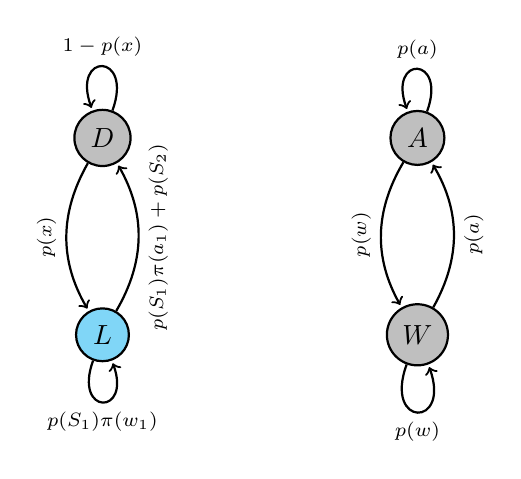
\begin{tikzpicture}[->,shorten >=1pt,auto,node distance=3cm,
                thick,main node/.style={circle,draw,font=\sffamily\Large\bfseries}]

            \node[fill=gray!50, circle, draw=black] (D) at (4,0) {$D$};
            \node[fill=cyan!50, circle, draw=black] (L) at (4,-2.5) {$L$};
            \node[fill=gray!50, circle, draw=black] (A) at (8,0) {$A$};
            \node[fill=gray!50, circle, draw=black] (W) at (8,-2.5) {$W$};

            \path[every node/.style={font=\sffamily\scriptsize}]
            (D) edge [in=110,out=70, loop] node[above] {$1-p(x)$} (D)
            (D) edge [bend right] node[above, rotate=90] {$p(x)$} (L)
            (L) edge [bend right] node[below, rotate=90] {$p(S_1)\pi(a_1) + p(S_2)$} (D)
            (L) edge [in=290,out=250, loop] node[below] {$p(S_1)\pi(w_1)$} (L)
            (A) edge [in=110,out=70, loop] node[above] {$p(a)$} (A)
            (A) edge [bend right] node[above, rotate=90] {$p(w)$} (W)
            (W) edge [bend right] node[below, rotate=90] {$p(a)$} (A)
            (W) edge [in=290,out=250, loop] node[below] {$p(w)$} (W);

        \end{tikzpicture}
    }
    \caption{\label{fig:partial_mps} Partial models for observations of light (left, MP1) and action (right, MP2). The transitions are derived from the original MDP (Fig. \ref{fig:delayed_mdp}) and weighted using its stationary distribution (Eq. \ref{eq:result_stationary_dist_mdp}).}
\end{figure}

\subsection{Block entropy curves} \label{ssec:res_block_entropy_curves}
We will now look at the block entropy behaviour of the previously obtained partial models, comparing it to the block entropy curves obtained by observations of the true MDP.
This will provide us with information about the adequacy of MP1 and MP2, showing if they are sufficiently complex to describe the MDP.
If they are, they could potentially be used by an agent to successfully learn the delayed action task.
In order to visualize the curves, we will choose the following numerical values for the free parameters:
\begin{equation}
    \label{eq:numerical_params}
    p(x)=0.6,\ \pi(a_0)=0.5,\ \pi(a_1)=0.3,\ \pi(a_2)=0.7.
\end{equation}

With this, we can calculate the stationary distributions of our processes, as well as the block entropy values for a given length, just by using the stationary distribution and the transition matrices to calculate the block probabilities (Fig. \ref{fig:block_curves}).
We can also calculate the final entropy rates for each system by using equation (\ref{eq:entropy_rate_MP}), which makes it possible to visualize the behaviour of convergence.

There is one elementary difference between the results obtained for MP1 or MP2 and the results for the MDP.
The results for the internal models can be seen as predictions the agent makes about its environment, while the results for the MDP are those that the agent obtains using observations.
This means that figure (\ref{fig:block_curves}) illustrates how predictions of the internal models compare to the real observations an agent would receive.

\begin{figure}[H]
    \centering
    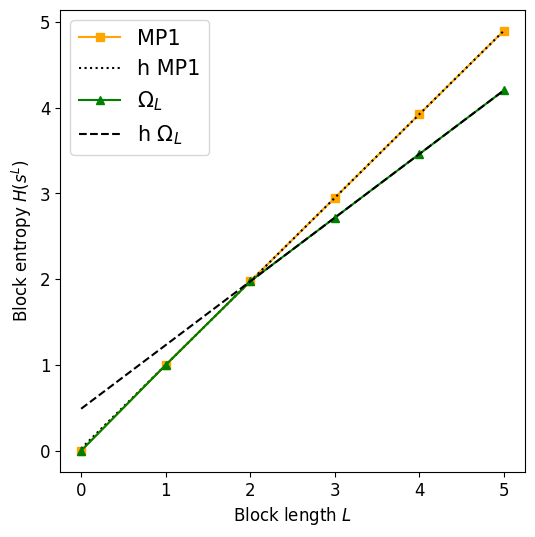
\includegraphics[width=0.49\linewidth]{../figures/mp1_obs_L_thesis.png}
    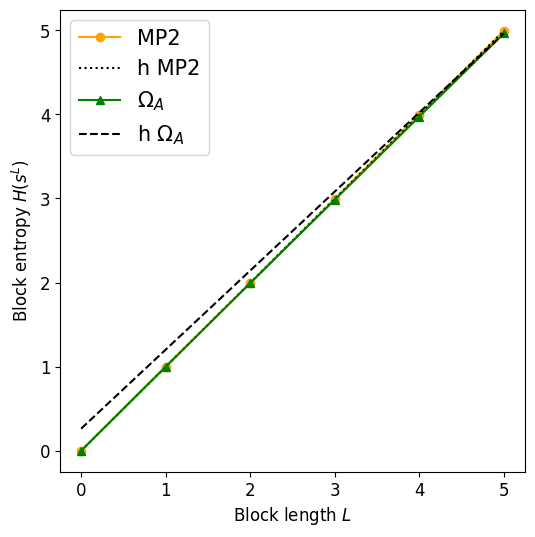
\includegraphics[width=0.49\linewidth]{../figures/mp2_obs_A_thesis.png}
    \caption{\label{fig:block_curves}Plots showing the block entropies of the partial models in orange (MP1 left, MP2 right) compared to the block entropies generated by observing the true MDP in green. The dashed and dotted lines show the final entropy rate to which the systems converge for the observations and the partial models respectively.}
\end{figure}

The first thing we can notice is that in both systems, there is a mismatch between the block entropies of sequences generated by the MDP (green triangles) and block entropies of sequences generated by the partial observation models (orange squares).
In case of the light (Fig. \ref{fig:block_curves} left), the difference is very distinct, showing a divergence exactly after $L=2$.
For the action (Fig. \ref{fig:block_curves} right) it is more subtle, but one can see that the two curves definitely start to separate at $L=5$.
There also are differences in how $\Omega_L$ and $\Omega_A$ converge to their respective final entropy rates $h\ \Omega_L$ and $h\ \Omega_A$.

The behaviours observed for $\Omega_L$ and $\Omega_A$ can both be explained with results from Crutchfield and Feldman \autocite{crutchfield2003regularities}.

Observing the light shows the block entropy curve of an order-R Markov Process, with R being the amount of states relevant for the transition probabilities of the next state.
The order of the process reflects in the point of synchronization, where the entropy rate reaches its final value.
This point is illustrated with the green points of $\Omega_L$ meeting the dashed line indicated by the final entropy rate of the observation $h \Omega_L$ (Fig. \ref{fig:block_curves}, left).
In our case, this implies R=2, where the entropy rate changes to match the black dashed line, meaning that the current state and the state before are needed to know the transition probabilities to the next state.

Looking at the structure of the delayed action task again (Fig. \ref{fig:delayed_mdp}), this result highlights how the light states are related to each other.
If an agent can only observe the current state of the light, $S_1$ and $S_2$ can not be distinguished since in both of them the light is on.
Yet, if the agent is able to look at the current state of the light and the state in the time step just before, it is possible to distinguish $S_1$ from $S_2$. 
Since $S_2$ is only reachable from $S_1$ and $S_1$ only from $S_0$, there must have been a light state before being in $S_2$ and a dark state before being in $S_1$.
This means that with $DL$ for $S_1$ and $LL$ for $S_2$ as distinguishable sequences, an agent capable of remembering the current state and the last one just before, so a temporal memory of length 2, would be able to distinguish all states of the MDP.

Comparing this behaviour to MP1, we can see that MP1 does not have any change in entropy rate $\Delta H(s^L)$, it matches the final block entropy (dotted line) already from the beginning.
Since $\Omega_L$ has exactly one change in entropy rate exactly at $L=2$, it signifies that there is some structure underlying the generating process that influences the block entropy for blocks of length 2, but no higher order complexity.
This means that MP1 does not have the order 2 complexity needed to accurately represent the light states of the MDP.

Yet it is interesting to note that MP1 and $\Omega_L$ do match in block entropy values for $L \leq 2$, suggesting that MP1 correctly models the behaviour of the MDP up to sequences of length 2.
This arises from how MP1 is computed, using the stationary distribution and transitions to the next state from the MDP, which implies accurate representation of blocks with $L\leq 2$.
It also means, that an agent with only the ability to look at blocks up to $L=2$ would not be able to see the shortcomings of MP1, seeing it as the correct model for this process.
This issue already shows an additional limitation for an agent trying to find the correct internal model from estimates with obtained observations, which will be discussed in section (\ref{sec:discussion}).
The choice of using stationary results of the MDP additionally implies inherent stationarity for MP1, explaining why it is already synchronized from the beginning.

When observing the actions of the agent, the behaviour can be characterized as that of a Hidden Markov Process.
This stems from the fact that in every state of the MDP, the agent will either act or wait, making the underlying states "hidden".
The convergence to the final entropy rate in this case is said to be exponential, implying complete synchronization only in the limit of infinity.
A visual result from this is that the block entropy of $\Omega_A$ will never match the dashed line of $h \Omega_A$, only asymptotically converge to it with every increase of $L$.
This means that there will always be some small uncertainty about the exact state of the system, even with many observed transitions.
In comparison to that, MP2 is again a model with no higher order structure, resulting in a straight line.
While this might not be easily visible in figure (\ref{fig:block_curves}), one can make the same argument as made for MP1, arguing that the way of creating MP2 results in a completely stationary process due to the stationary distributions and transitions used from the MDP.

Regarding the accuracy of MP1 and MP2 as models of the true MDP, we can now conclude that both are not exact representations of the underlying MDP.
This can also be understood as the internal model predicting a certain behaviour, the orange values, but failing at matching the observations in green, implying that the current internal model is not sufficiently complex.

\subsection{A sufficiently complex internal model} \label{ssec:sufficient_internal_model}
In the case of observing the light state in the delayed action task, synchronization has been shown to be achieved at finite block lengths, specifically $L=2$.
Using this information, we can create a model using length 2 blocks as states (Fig. \ref{fig:mp1_L2}).

% L=2 light process
\begin{figure}[H]
    \hspace{2cm}
    \resizebox{0.58\linewidth}{!}{
        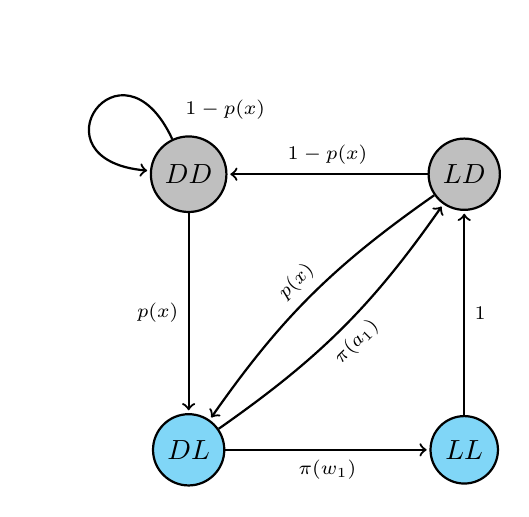
\begin{tikzpicture}[->,shorten >=1pt,auto,node distance=3cm,
                thick,main node/.style={circle,draw,font=\sffamily\Large\bfseries}]

            \node[fill=gray!50, circle, draw=black] (DD) at (0,3.5) {$DD$};
            \node[fill=gray!50, circle, draw=black] (LD) at (3.5,3.5) {$LD$};
            \node[fill=cyan!50, circle, draw=black] (DL) at (0,0) {$DL$};
            \node[fill=cyan!50, circle, draw=black] (LL) at (3.5,0) {$LL$};

            \path[every node/.style={font=\sffamily\scriptsize}]
            (DD) edge [in=175,out=115, loop] node[right=1cm] {$1-p(x)$} (DD)
            (DD) edge node[left] {$p(x)$} (DL)
            (DL) edge [bend right=10]  node[below, rotate=45] {$\pi(a_1)$} (LD)
            (LD) edge [bend right=10]  node[above, rotate=45] {$p(x)$} (DL)
            (LD) edge node[above] {$1-p(x)$} (DD)
            (DL) edge node[below] {$\pi(w_1)$} (LL)
            (LL) edge node[right] {$1$} (LD);

        \end{tikzpicture}
    }
    \caption{\label{fig:mp1_L2} Internal model with sufficient complexity to explain the light state of the delayed action task, created using length 2 blocks as states.}
\end{figure}

An internal model of this form would be sufficient for the agent to synchronize to the MDP, potentially making it possible to learn the optimal policy for the delayed action task.

\subsection{Estimating block entropy and predictability gain} \label{ssec:est_block_and_pred_gain}
Now knowing the analytical result for the necessary complexity of the internal model, we want to further investigate how an agent would be able to come to this conclusion by itself.
We will only analyse the case of observing the light now, since the desired complexity is reachable with finite block length.
The agent would have to estimate the predictability gain for the incoming observation in order to find the block length needed to accurately represent the observation.

To simulate the estimation process for the delayed action task, 1000 replications using sequences of length 50 were computed using the transition matrix of the MDP (Eq. \ref{eq:P_mdp}), using the MDP stationary distribution (Eq. \ref{eq:result_stationary_dist_mdp}) to initialize each sequence.
The sequences were reduced to the light observations (see section \ref{ssec:observing_mdp}) and block entropy values were then estimated using equation (\ref{eq:plug_in_block_ent}).
The resulting values can then be compared with the analytical results from before (Fig. \ref{fig:entropy_est}).

\begin{figure}[H]
    \centering
    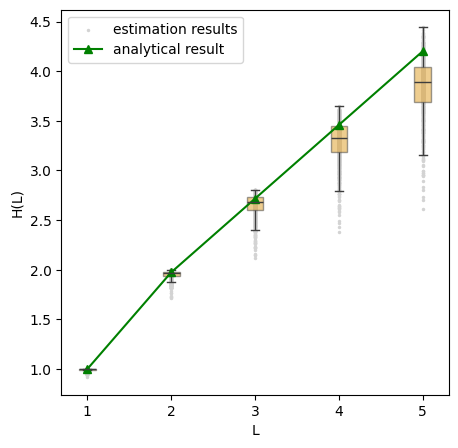
\includegraphics[width=0.6\linewidth]{../figures/block_entropy_estimation_thesis.png}
    \caption{\label{fig:entropy_est} Plot showing the results when estimating block entropy from sequences of length 50. The histograms show the combined results from 1000 replicates.}
\end{figure}

One can see that the estimate of the block entropy becomes worse for larger block lengths, not only having higher variance, but also resulting in values further below the analytical results.
This is in part due to the nature of the used plug-in-estimator, which is known to underestimate the true result for finite sample size, which is also called negative bias \autocite{basharin1959plugin}.
A more dominant reason here though is the temporal correlation between samples, since samples come from the same trajectory of the MDP for each sequence.

When estimating the predictability gain, this issue with bias and variance has significant implications for the results the agent obtains.
Since the needed complexity is determined by the last block length with non-zero predictability gain, negative bias will wrongly shift the complexity estimate to higher block lengths, as seen in figure (\ref{fig:pred_gain}).
This means that the agent would estimate the system to be more complex than it actually is.

\begin{figure}[H]
    \centering
    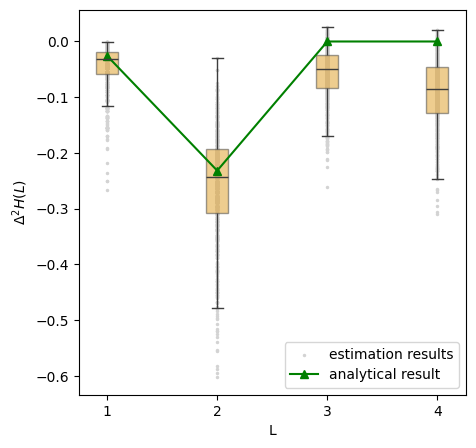
\includegraphics[width=0.6\linewidth]{../figures/predictability_gain_thesis.png}
    \caption{\label{fig:pred_gain} Plot showing the estimated predictability gain for sequences of length 50. The histograms show the combined results from 1000 replicates.}
\end{figure}

Nicely enough, the plug-in-estimator is a consistent estimator, implying that with sequence length approaching infinity, the bias and variance will vanish, making the estimate converge to the analytical result \autocite{basharin1959plugin}.
While infinite sample size is of course not feasible for any agent, it would also be desirable in general to have a minimal sample size, since this would make the agent more efficient.
The simulations here are just a demonstration of the difficulty encountered when trying to estimate the complexity of an observation.
More analysis would need to be done to see how exactly this estimation could be implemented efficiently for use in an agent.


\newpage
\section{Discussion} \label{sec:discussion}
The results presented show that information theoretical measures can be applied to a Partially Observable Markov Process in order to find sufficiently complex internal models, though mostly analytically.
From observing the light state of the system, one can obtain an internal model which is sufficiently complex to explain the observed block entropy of the light state.
The found representation does not correctly reflect the true MDP though, i.e. with four states instead of three.

Other work by Crutchfield shows that for unifilar processes, in which each state only emits distinct symbols, once a sufficiently complex model is found, the true system can be recovered by correctly reducing the model if necessary.
This model is then called the $\epsilon$-machine of the system \autocite{crutchfield1994calculi}.
A proposed way to reconstruct the $\epsilon$-machine of a system is to iteratively increase model complexity based on the incoming observations.
This procedure could also be implemented for the delayed action task.

It has also been shown that this procedure can be used for Hidden Markov Processes \autocite{jurgens2021HMP}.
This means that the action of the agent could also be modelled with an $\epsilon$-machine, potentially enabling the agent to infer the impact of its actions in relation to the light state by using states which combine light state and action.
With this, an agent might be able to infer the optimal policy just from its internal model without having to learn the policy directly, as in other approaches of reinforcement learning like q-learning.
It may also enable the agent to simulate the environment by itself, which could be used to improve the policy similarly to methods in Projective Simulation \autocite{briegel2012ps}.

For this, further work would need to be done to clarify the difficulties in estimation shown in section (\ref{ssec:est_block_and_pred_gain}).
There are papers which propose certain thresholds for sequence lengths in order to mitigate bias and get sufficiently accurate results.
\autocite{lesne2009entropy} show that the needed sequence length $N$ to accurately estimate block entropy of length $n$ with $k$ symbols depends on the final entropy rate $h_\mu$:
\begin{equation}
    \label{eq:lesne_seq_length}
    n \leq \frac{N h_\mu}{\ln(k)}.
\end{equation}

They propose first estimating the entropy rate using Lempel-Ziv complexity, which is not biased in the same way as the plug-in-estimator, then selecting the sequence length accordingly.
Other works use slightly different sequence lengths, but all of them incorporate the influence of $h_\mu$ into their results \autocite{larson2011block,dkebowski2016consistency}.

It should also be possible to calculate confidence intervals for the estimates, providing additional information for the agent.
Estimation is a major point of concern in this framework and should be addressed more thoroughly in future work.

It is important to note that the result of this estimation now strongly depends on the capacity of the agent to store long sequences.
Depending on the length of memory, high block lengths can not be estimated confidently.
This also means that if the memory is too short, an agent is not able to find the highest order complexity for a given sequence.
If, for example, only blocks up to $L=2$ could be estimated by an agent observing the light state of our delayed action task, the agent would not find an accurate model.
It would actually find MP1 do be an accurate representation, since it matches blocks entropies up to $L=2$.
This means that an agent will converge to an insufficient internal model, if the length of observed sequences is too short compared to the complexity of the generating process.

One way for the agent to be aware of this limitation would be to estimate a final entropy rate $\hat{h}_\mu$ for the internal model and compare it to the one used to determine sequence length.
The difference between those values would tell the agent how far the internal model is away from an accurate representation, even if the current model is the optimal one for the obtainable sequence length.

\newpage
\section{Conclusion} \label{sec:conclusion}
Creating more realistic and capable artificial agents promises a more complete understanding of agency and the emergence of complex behaviour in complex adaptive systems.
It has been shown that information theory is a very powerful tool, which can be used to infer a lot about a system even in circumstances with limited information.

The model-based approach shown here has the potential to provide strong methods for policy optimization, with additional adaptability due to a dynamic, iterative approach to internal model generation.
Current methods for solving POMDPs usually rely on a correct internal model to begin with, which would make the proposed framework a huge improvement in terms of adaptability and usefulness.
With internal models representing the observed environment, this approach offers an excellent way to study the learning process of agents, clearly illustrating the structures an agent is able to identify from its own experiences.

In order to prove the viability of this framework, more work has to be done to show how exactly it can be realized and deployed in an agent.
The potential benefits give strong motivation to pursue more research focused on internal model generation.

\section{Acknowledgements} \label{sec:acknowledgements}
I would like to thank Hans Briegel for making a thesis in this research area of his group possible, as well as Alexander Vining for providing me with this incredibly interesting topic and the support throughout.
I was able to learn about an extremely fascinating, and in my opinion very relevant area of research with great future potential.

\clearpage
\section*{Declaration of Authorship}

I hereby solemnly declare, by my own signature, that I have independently authored the presented work and have not used any sources or aids other than those indicated. All passages taken verbatim or in content from the specified sources are identified as such.

I consent to the archiving of this Bachelor thesis.

\hfill
\vspace{2cm} Innsbruck, \findate \hfill Lukas Prader \includegraphics[height = 10mm]{"signature.png"}


\newpage
\printbibliography[]
\newpage
\appendix



\end{document}